%%%%%%%%%%%%%%%%%%%%%%%%%%%%%%%%%%%%%%%%%%%%%%%%%%%%%%%%%%%%%%%%%%%%%
% LaTeX Template: Project Titlepage Modified (v 0.1) by rcx
%
% Original Source: http://www.howtotex.com
% Date: February 2014
% 
% This is a title page template which be used for articles & reports.
% 
% This is the modified version of the original Latex template from
% aforementioned website.
% 
%%%%%%%%%%%%%%%%%%%%%%%%%%%%%%%%%%%%%%%%%%%%%%%%%%%%%%%%%%%%%%%%%%%%%%

\documentclass[12pt]{article}
\usepackage[a4paper]{geometry}
\usepackage[myheadings]{fullpage}
\usepackage{fancyhdr}
\usepackage{lastpage}
\usepackage{graphicx, wrapfig, subcaption, setspace, booktabs}
\usepackage[T1]{fontenc}
\usepackage[font=small, labelfont=bf]{caption}
\usepackage{fourier}
\usepackage[protrusion=true, expansion=true]{microtype}
\usepackage[english]{babel}
\usepackage{sectsty}
\usepackage{url, lipsum}
\usepackage[table,xcdraw]{xcolor}
\usepackage{float}


\newcommand{\HRule}[1]{\rule{\linewidth}{#1}}
\onehalfspacing
\setcounter{tocdepth}{5}
\setcounter{secnumdepth}{5}
\graphicspath{ {./Images/} }

%-------------------------------------------------------------------------------
% HEADER & FOOTER
%-------------------------------------------------------------------------------
\pagestyle{fancy}
\fancyhf{}
\setlength\headheight{15pt}
\fancyhead[L]{APS490: Final Report}
\fancyhead[R]{University of Toronto}

%-------------------------------------------------------------------------------
% TITLE PAGE
%-------------------------------------------------------------------------------

\begin{document}
\pagenumbering{gobble}
\title{ \normalsize \textsc{APS490 - Bombardier Capstone Project}
		\\ [2.0cm]
		\HRule{0.5pt} \\
		\LARGE \textbf{\uppercase{Universal Calibration Block \\}}
		\LARGE Bombardier Aerospace
		\HRule{2pt} \\ [0.5cm]
		\normalsize \today \vspace*{5\baselineskip}}

\date{}

\author{
		Abhinav Ramakrishnan (999122514) \\  
		Jonathan Ramoutar (998838003) \\ 
		Miaoyi Lu (998552070) \\
		Nisitha Jayatilleka (998907928) }

\maketitle
\newpage
\section*{\textsc{Executive Summary}}

The clients of the project, Alex Vinitsky, Jackie Yu, and Teodora Patrasc, are engineers in Bombardier Aerospace's De Havilland location's In-Service Engineering Structures department. They request a universal calibration block to replicate a variety of repair configurations of Dash-8 commercial airplanes. This project requires consideration of: airplane structure and components; Non-Destructive Testing (NDT) with eddy currents; and fatigue of the frames, stringers, and fuselage skin. 

Functions, constraints, and objectives are defined to scope the project and to meet the requirements of the stakeholders. The primary function is the replication of defects and repair configurations to allow for calibration. The objectives recognized are safety, low cost, portability, ease of use, reliability, traceability, ergonomics, robustness, and manufacturability. The project is also constrained by manufacturing expense and the required versatility in covering 50\% of the possible repair configurations and crack locations. In addition the design has to be compliant with regulations in the AM \& M (Air-craft Maintenance \& Manufacturing) standards prescribed by Transport Canada.

A broad spectrum of suitable machining tools/methods, methods for the creation of cracks, and manufacturing of skin layer and doublers, were researched. The team decided to adopt EDM as the preferred method of defect creation and CNC machining as the preferred method of fabrication. Based on the research conducted three designs were proposed. `The Staircase' design constitutes having discrete thicknesses of the skin layer and the doubler, each mounted on top of each other by rivets. `The Hook' design is a variant of the idea that a crack can be simulated by pressing two plates together. `The Petri Dish' is a design where a series of skin layers and doubler layers can be stacked on top of each other to create a versatile system that can replicate different thicknesses.

Finally, the constraints and objectives were prioritized and given a normalized grading system. It is seen that low cost and reliability are the high priority objectives the design should meet. Utilizing these weights in a weighted sum model, a rigorous analysis was done in order to compare the designs to each other and against the objectives. After the analysis, it is found that the `Staircase' design is the best design to be implemented. Upon the client's suggestions the design was then improved. 

A cost analysis of the `Staircase' was performed, and the final design is estimated to have the total cost of manufacturing and raw material be \$2608.18, which is less than the cost of manufacturing existing Bombardier Aerospace design: \$3000. Finally, and a design for removable fasteners made from countersunk rivets with threading were implemented. 
\newpage

\renewcommand{\contentsname}{\textsc{Contents}}
\newpage
\textsc{\tableofcontents}
\newpage

%-------------------------------------------------------------------------------
% Section title formatting
\sectionfont{\scshape}
%-------------------------------------------------------------------------------

%-------------------------------------------------------------------------------
% BODY
%-------------------------------------------------------------------------------

\pagenumbering{arabic}
\fancyfoot[R]{Page \thepage\ of \pageref{LastPage}}
\section{Problem Statement}
%\addcontentsline{toc}{chapter}{Problem Statement}
Alex Vinitsky, a principal engineer at Bombardier Aerospace's De Havilland location, has asked for a standardized means of calibrating eddy current probes for non-destructive testing of airplane repairs. He, Jackie Yu (structural repair engineer), and Teodora Patrasc (senior NDT specialist, level III), request that a universal calibration block be made to be used for many different repair configurations.

The In-Service Engineering Structures department at Bombardier offers repairs for damages on their air-crafts reported by operators. Often these repairs - in particular, repairs for damage on fuselage skin - require the operators to inspect for crack damage, usually through eddy current probing. The airlines and operators usually outsource this task and call in level I or level II NDT specialist inspectors. The inspectors calibrate their probing equipment using calibration blocks that replicate the material, design, and thickness of the repair area. As such, individual calibration blocks have to be acquired for different parts of the aircraft. The blocks have manufactured approximations of cracks and defects in locations where such damage is expected. It is costly and difficult to obtain individual calibration blocks that replicate all of these factors. Universal calibration blocks are desired to ease this replication process: they are however costly to create. Compromising design aspects for cost leads to fewer applicable configurations. 

The team (comprising of Abhinav Ramakrishnan, Nisitha Jayatilleka, Jonathan Ramoutar, and Clover Lu) is asked to design a product that applies to many repair configurations for Bombardier's Dash-8 commercial airplanes. This universal block will be made with consideration for the identified concerned parties, and it will include the design elements outlined in this report.
\newpage
\section{Background}
%\addcontentsline{toc}{chapter}{Background}

The following subsections expand on the nature of this project, providing context to the requirements of the design. It is necessary to expound upon the nature of the aerospace industry, fracture/fatigue analysis, and NDT methods - specifically eddy current testing. This information lends to the definition of the functionality and use of the expected design.

\begin{figure}[h!]
  \centering
  	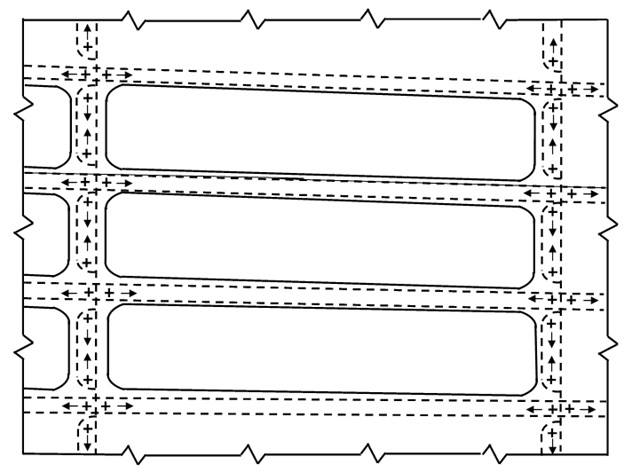
\includegraphics[width=\textwidth]{image1}
  \caption{Diagram of the average Q400 fuselage skin assembly}
  \label{fig:fig1}
\end{figure}	

In order to clarify terms used in these subsections, Fig. \ref{fig:fig1} was drawn to illustrate certain airplane components. The figure depicts fuselage skin: three bays between two frames and four stringers. The frames span the fuselage circumference (vertically in the diagram) and run from the front to the back of the plane (horizontally in the diagram). Stringers run laterally and are placed circumferentially. The solid lines within the diagram indicate the outline of the chem-milled pockets (a feature not found on the Q100, 200, and 300 crafts).
 

\subsection{\textsc{Industry}} 

The aircraft industry has advanced a lot in the past century, and with these advancements a variety of methods for Non-Destructive Testing (NDT) have surfaced. The main methods of testing used currently are:

\begin{itemize}
\item Eddy Current Testing
\item Ultrasonic Testing (mostly used to check for waffle dis-bonding)
\item Visual Inspection
\item Radio-graphical Testing
\item Fluorescent Penetrant Testing
\item Magnetic Particle Testing
\item Resonant Frequency Testing
\end{itemize}

All of these methods have their individual advantages and disadvantages, but, as Bombardier has placed an emphasis on low frequency (sub-surface) eddy current inspection, the team will focus on this method of NDT as requested by the client.
 
\subsection{\textsc{Eddy Current}}

\begin{figure}[h!]
  \centering
  	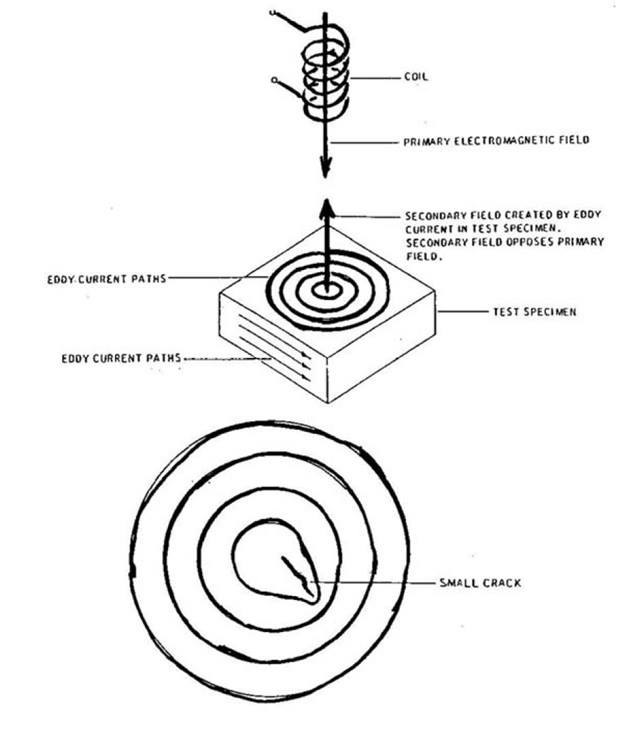
\includegraphics[width=0.75\textwidth]{image2}
  \caption{(Top) Generation of eddy currents in the object. (Bottom) Distortion of eddy currents due to defects. Figure taken from [1].}
  \label{fig:fig2}
\end{figure} 

Eddy current testing is widely used to detect surface/pseudo-surface (minimally buried) defects. This method is applicable only to electrically conductive materials. For eddy current testing, an object is brought close to an alternating current (AC) carrying coil. This produces an alternating magnetic flux which induces closed loop circulating currents (called eddy currents) in a plane perpendicular to the magnetic flux. The eddy currents in turn generate a magnetic flux that counters the inducing magnetic flux, thus lowering the current in the AC coil. This reduction in current (magnitude) is measured along with the change in phase and both are displayed graphically on the probe/scope. If a fault exists, then, depending on the size and depth of the fault the eddy currents develop particularities in magnitude and phase indicative of the faults orientation and location [1]. One of the important elements affecting eddy current signals is the coupling between the object and the probe, which translates as a unique signal occurring when the probe is removed from an object with no faults: the lift-off signal. The eddy current methodology is illustrated in Fig. \ref{fig:fig2}.

\subsection{\textsc{Fractures}}\label{sec23}

Fatigue is the process of initiation and propagation of cracks as a result of cyclic loading. Since airplanes are subjected to cyclic loading fatigue cracks are prominent and detecting and repairing these cracks is an important part of the servicing process. As described in the previous section the client, Bombardier, uses the eddy current method to detect these cracks. The types of materials commonly used and the crack propagation in each will be addressed briefly in this section.

Fatigue life of metals and alloys can be broken down into several sections: crack nucleation, micro-crack growth, macro-crack growth, and failure. 

Crack nucleation (the initiation of the crack) is aided by the presence of inclusions or voids present in engineered materials. Aluminum Alloy 7075-T6 and Aluminum Alloy 2024-T3, used by Bombardier for the stringers and frames, and the skin and repair doublers fall under this category. 

Crack growth from voids, inclusions, or slip-bands within the range of 1 to 20 $\mu$m in length fall under micro-crack growth or small-crack growth. A crack growth of 100$\mu$m is shown to take up to about 80\% of the fatigue life [2] for commercial alloys. Micro-cracks are not within the scope of this project as the client is concerned with detecting cracks which are $\frac{1}{4}$ in. (6.35 mm) in length and 0.004'' in width.

Macro-crack propagation (>20 $\mu$m) has been studied extensively in the aerospace industry. This is due to the fact that detection of macro-cracks is what denotes the necessity of repairs. Specific studies and flight simulation tests have been carried out on the aforementioned alloys [3][4][5]. Shown below is an illustration of the typical variation in crack growth rates. It is important to realize that the cracks within the scope of this project occur within the mid-section of the graph below.

\begin{figure}[H]
  \centering
  	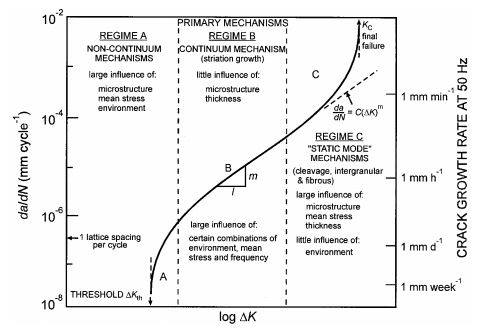
\includegraphics[width=0.95\textwidth]{image3}
  \caption{Schematic illustration of the typical variation in fatigue-crack growth $\frac{da}{dN}$, as a function of the applied stress-intensity range $\Delta K$ in metallic materials, showing the regimes of primary growth-rate mechanisms and effects of several major variables on crack-growth behavior.}
  \label{fig:fig3}
\end{figure}

This fatigue analysis is a key component of the work done in the ISE Structures department at Bombardier. The repair information is issued and if need be inspection intervals are also prescribed as per the calculated life of repair, measured in flight cycles[3]. One such repair that requires these types of inspections is the installation of a repair doubler or repair joint. Here, a doubler is defined as an additional layer of material fastened over damaged airplane skin by way of rivets. (A joint is similar to a doubler with a few key distinctions, the biggest being that a joint carries load while a doubler does not.) During the installation process and over the course of the craft's life it is necessary to check for cracks near the repair that indicate fracture failure. Because the repair doubler is covering an additional layer of skin, some cracks may exist that cannot be found through visual inspection. Hence, to avoid undoing the repair, and to avoid finding the defect location from the inside of the airplane (after removing interior hardware and furnishing), non-destructive testing is used.
\newpage
\section{Stakeholders}

These stakeholders and their requirements were identified through communications with the client (seen in the Appendix) and through researching NDT method regulations as they pertain to the aerospace industry.

\begin{itemize}
\item Bombardier (Mr. Vinitsky, Ms. Patrasc, Mr. Yu)\hfill \\
The product directly influences Bombardier Aerospace and the department at which Mr.Vinitsky, Ms. Patrasc, and Mr. Yu work. Therefore the primary stakeholders are our clients, including the whole of Bombardier Aerospace, which they represent.

Stakeholder Requirements: 
\begin{itemize}
\item The design should emulate possible cracks on Bombardier air-crafts.
\item The product less expensive than the current product.
\item The product functions varying thicknesses of the aircraft fuselage components.
\item The product functions for different repair configurations.
\end{itemize}

\item End users \hfill \\
The end users are the people who interface with the product and depend on its results being accurate. This includes plane operators, structural engineers, and maintenance \& repair workers amongst others.
 
Stakeholder Requirements:
\begin{itemize}
\item The product should emulate detectable cracks within the required precision 
\item Features and structure of the product should meet safety standards at Bombardier. 
\item The design should be easy to use, thus saving time and cutting back on frustration from arduous tasks.
\end{itemize}

\item Transport Canada Aircraft \hfill \\
Transport Canada Aircraft is a government overseeing institution that sets regulations and standards on how airplanes are to be inspected, maintained, and manufactured. Transport Canada will be considered  as a secondary stakeholder.

Stakeholder requirements:
\begin{itemize}
\item Transport Canada requires that the  Aircraft Maintenance \& Manufacturing (AM \& M) regulations are met such that the airplanes are airworthy.
\end{itemize} 

\end{itemize}
\newpage
\section{Project Scope}
%\addcontentsline{toc}{chapter}{Project Scope}

The following functions, objectives, and constraints define the scope of the problem. The team came up with their own set of functions, objectives, and constraints separately, and then discussed the results. Common identified functions between team members were prioritized; unique items were scrutinized through discourse until a consensus was reached as to the importance of that function. Objectives were listed and rated by each member from 1 (least important) to 5 (most important), allowing the average scores to dictate which objectives were primary. 

\subsection{\textsc{Functions} }

\textbf{Primary Functions:}

\begin{itemize}
\item Allow for the calibration of eddy current probes: Give appropriate lift-off signals and signals that indicate crack locations.
\item Replicate cracks to the required precision.
\item Replicate different repair configurations of Bombardier air-crafts.
\end{itemize}

\noindent
\textbf{Secondary Functions:}

\begin{itemize}
\item Allow to simulate data of aircraft damages for study.
\item Allow for training demonstrations for new plane operators and maintenance \& repair workers.
\end{itemize}

\subsection{\textsc{Objectives} }
\begin{itemize}

\item Safety \hfill \\ 
The new products will be handled by operators and inspectors at Bombardier Aerospace and related airlines. The safety of the operators will be considered when designing the calibration block. Thorough training on the use of these blocks will be provided, however, designing for safety does not need to be overly prioritized in the event of other objectives being missed.

\item Low cost \hfill \\
One of the main concerns of the client is the cost of the product. The existing equipment is non-modular, meaning that in the event of a defect the calibration blocks will be replaced entirely resulting in a high cost for the clients. This is the main reason for the need of a new calibration block and as such it is a high priority objective.
		
\item Portability \hfill \\
As the calibration blocks are to be used on-site it is important that they are portable in the sense that they can be carried without issue between storage and hangar bays, and around the repair area. This will facilitate ease of use. Compactness of the design should be considered with possible adverse effects on ease-of-use: compact designs might require significant reassembly before utility.

\item Ease of use/Clarity/Simplicity \hfill \\
The final product should be easy to use and understand, the main objective being that Bombardier will not have to spend excessive amounts of resources to train its employees to use the product.

\item Reliability \hfill \\
The product has to replicate fractures reliably. This will also be listed as a constraint due to its importance, owing to the fact that detecting fractures in an airplane is of utmost priority as this will be a crucial factor in determining the safety of operating the airplane.		

\item Traceability \hfill \\
In order to ensure that the product and every detachable piece therein do not get lost every detachable piece of the product and the product itself would be benefited by having unique identifying numbers. 

\item Ergonomics \hfill \\
A design that considers human ergonomics will be preferred. For example, it is very possible that  a significant portion of end users will be left handed - thus a design that satisfies Left-Right Mirror Neutrality will be objectively superior.

\item Robustness \hfill \\
The product should have a comparable life cycle to that of the current implementation. As such, wear and tear of the product (i.e. design for minimum moving parts) will be considered during the design phase.

\item Manufacturability \hfill \\
Should the design be successful and meet expectations, Mr. Vinitsky and the team at Bombardier hope to produce these calibration blocks on a mass scale and offer them to the operators and inspectors in the many commercial airlines that make up their customer basis. As such the product should be easy to mass produce. 
\end{itemize}


\begin{table}[h!]   
\begin{center}
    \begin{tabular}{ | l | c | c | c | c | c |}
    \hline
    Selection Criteria & Avg. Weight & Member 1 & Member 2 & Member 3 & Member 4 \\ \hline
    Low Cost & 5 & 5 & 5 & 5 & 5  \\ \hline
    Safety & 2.5 & 1 & 5 & 2 & 2  \\ \hline
    Portability & 3 & 3 & 3 & 2 & 4  \\ \hline
    Ease of Use & 3 & 2 & 3 & 4 & 3  \\ \hline
    Reliability & 4.75 & 5 & 4 & 5 & 5  \\ \hline
    Traceability & 2.5 & 3 & 3 & 2 & 2  \\ \hline
    Ergonomics & 1.5 & 1 & 2 & 2 & 1  \\ \hline
    Robustness & 2.75 & 4 & 2 & 2 & 3  \\ \hline
    Manufacturability & 3 & 2 & 3 & 2 & 5  \\ \hline
	\end{tabular}
\caption{Table showing the importance that each team-member ascribed to a given objective}    
\end{center}
\end{table}

\subsection{\textsc{Constraints}}
\begin{itemize}

\item Cost \hfill \\
The cost of the new product is limited by Bombardier Aerospace's currently implemented solution: the cost of a single unit should be less than CAD 3000 (ignoring economies of scale).

\hskip 15pt 
Calibration blocks are expensive to create mostly due to the creation of defects against which the probe is calibrated. The cracks must be as thin or as fine as possible and must span the minimal detectable length of a crack defined by Bombardier and the aerospace industry (as stated in Section \ref{sec23}, typically a quarter of an inch or one rivet pitch). Methods such as Electric Discharge Machining can be used to create thin cuts that approximate cracks, but apart from the fact that the thinness of the cuts is limited by the width of the wire, this process is costly. Other methods include pushing two plates together to recreate thin cracks (although the cracks are then ``infinitely'' long), and actually fatiguing the part to failure (which is both very costly and time consuming). 

\hskip 15pt 
With the current design of the calibration blocks individual blocks are necessary to replicate different parts of the fuselage. The new design is expected to cut back on the cost by having a universal calibration block which can replicate several configurations and thereby reducing the number of blocks needed. Modularity will be considered during the design phase as this will allow for better serviceability. For example, a damaged part could be replaced without having to replace the entire calibration block.

\item Versatility \hfill \\
As per design requirements from Bombardier the proposed design must cover roughly 90\% of the possible repair configurations and crack locations. Repair configurations are numerous and deal with many different factors. A repair on the fuselage can be overtop the craft skin, as well as underlying structural elements like stringers and frames. Defects may exist in any or all of these layers. A doubler may be placed near a window cutout or a cutout for the baggage door assembly - these repairs require different testing specifications, i.e. different calibrations. As well, since eddy current testing differs based on the materials in use, the calibration blocks need to account for material. Furthermore they must also account for the fact that different chromate-coatings affect the probe signal. All of these configurations can also be done with a wide range of doubler thicknesses over a range of skin thicknesses; this needs to be accounted for, too. 

\item Regulatory Compliance \hfill \\
The design has to meet AM \& M standards prescribed by Transport Canada. These standards exist to ensure that products built for aeronautical use - operated or maintained under Canadian control - meet national and international airworthiness standards.

\end{itemize}
\subsection{Summary of Design Requirements}

The final product is expected to simulate at least 50\% of the repair configurations. These configurations include: fuselage-skin and repair doubler atop the fuselage, repairs near the aft baggage door, and repairs near the window and the door cutout of the `Dash-8' planes (the Q100, 200, and 300 series, as well as the Q400 series). The repair configurations can also vary according to rivet size and type, crack location, repair location, and the inclusion of structural elements such as stringers and frames. 
\newpage
\section{Analysis of Manufacturing and Fabrication Methods}
\subsection{\textsc{Crack creation or manufacturing of cracks}}

Ideas and available methods regarding the manufacturing of cracks will be discussed in this section. These are not the only options available, however other methods have been disregarded as they have been deemed unfeasible. For example, it is possible to create notches in a part and subject the part to fatigue until a crack is generated - however, the costs of accomplishing this are much greater than for the methods below.

\subsubsection{Laser Cutting}
A highly focused laser beam is directed at the metal piece. This will effectively melt and evaporate the metal. This method gives relatively smooth crack walls. Laser beam cutting has an accuracy of around $\pm$0.025 mm and can cut into 6.35 mm mild steel. The width of the crack can be adjusted by focusing the beam. As the accuracy required to simulate the cracks is around 0.004 inches (0.1 mm), and the depth of crack does not exceed 1 mm, laser cutting is a viable means of generating the cracks.

\subsubsection{Electric Discharge Wire-Cutting}
This is a variation of Electronic Discharge Machining (EDM). Here a high current is passed through a wire which is in turn used to cut through the part. The part itself is mounted on a milling machine. As the part is maneuvered the wire cuts through the metal. The accuracy of this method is comparable to that of laser cutting and is around $\pm$0.025 mm.The crack walls are similarly smooth when compared to laser cutting. The average cost of creating a notch using EDM is approximately \$75 .

\subsubsection{Aluminum PAN etching}
Theoretically it is possible to place a positive photo-resist on the aluminum part (thereby covering it completely) and then expose it using UV photo-lithography [6]. This generates a pattern on the surface of the photo-resist after it is washed with the requisite solvent. After generating the pattern we may then use an aluminum PAN (Phosphoric - Acetic - Nitric) solution to etch the pattern onto the surface of the part. The PAN etch does not typically have any noticeable effect on the photo-resist. The time submerged in the PAN etch decides the depth of the pattern [7]. The accuracy of this method is on the order of a hundred nano-meters (the wavelength of the light used). The cost of this method is usually around \$160 for creating the mask and approximately \$40 to acquire the materials for the photo-resist and the PAN solution. The price does not change significantly with the number of cracks to be generated since all these processes can be done in batches. The cost of using the machines involved is dependent on the number of hours of machining - at the University of Toronto the cost is \$32 per hour of use (capped at \$350 per month).

\subsubsection{Adjacent sheets}
Pushing two metal sheets of equal thickness together is a way of simulating a finer crack than by machining. The length of the crack simulated is then equal to the length of contact between the two sheets. This means that creating cracks within a layer of metal - that are not edge cracks or that do not cleave the layer completely - is difficult. The `Hook' design provides a possible solution to this. This method is still useful in that it does not include any additional costs beyond the machining of the plate geometries.

\subsubsection{Preferred Method of Defect Creation}

Out of the listed crack manufacturing methods EDM appears to be the best method, as it is less costly than laser cutting and PAN etching (\$400/hour at University of Toronto). The adjacent sheets method suggested by the team does not serve as well since the cracks created through this method are too long. (It should be noted that, while `The Hook' design attempts to rectify this, the geometry and assembly require tight tolerances, leading to increased fabrication costs).


\subsection{\textsc{Fabrication of the Calibration Block}}
Manufacturing and assembly methods for the calibration blocks will be discussed here. These methods address the means of creating the metal plates that represent the fuselage skin, repair doublers, and the various thicknesses of both.  Special consideration is given to the surface quality of the machined parts, and the accuracy of the machining method. 

\subsubsection{Computer Numerical Control (CNC)}
CNC machining is one of the most popular types of machining in the industry. Fundamentally this can be described as a computer guided milling process. Due to the application of an automated control system, most human errors and inaccuracies that occur during manual machining are avoided. CNC machining provides a fast and accurate method of machining. The total machining costs have been estimated to be upwards of \$200 [8].  

\subsubsection{Chemical milling}
This method uses baths of etching chemicals to create a necessary shape. A corrosive chemical reagent called an `etchant' is applied over the areas where the material needs to be removed. The etchant reacts with the material and dissolves the surface. Inert chemicals are applied over non-etch surfaces [9].

\subsubsection{Gel/Tape Adhesion}
A simulation of one thickness of material can be created by joining together many thinner sheets by placing one on top of the other, hence totaling up to the required thickness. However there exist air gaps between the thinner layers which reduce the probing depth and amplitude of the eddy current, weakening the signal being read. As a solution, a gel/tape with comparable conductivity to the material of the block itself is suggested for application between the layers. In other words, in lieu of an air interface there is now a gel/tape interface. This is used in the proposed `Petri-Dish' design.

\subsubsection{Preferred Method of Fabrication}
The team decided that CNC Milling is the best method to manufacture the structure as it is the cheapest in comparison to the other two methods (costing: \$ 206.25). There are also significant disadvantages to the two other methods. Chemical Milling can be hard to control and the level of accuracy required might be hard to achieve. Gel/tape adhesion, whilst innovative, is untested and would be hard to get accredited by an official agency. Further, there is the issue of significant loss at the metal-metal interface which could cause unpredictable phase/amplitude fluctuations in the eddy signal. 
\newpage
\section{Proposed Designs}
%\addcontentsline{toc}{chapter}{Stakeholders}
The following alternative designs were created upon consideration of the processes described later in detail in Section 5. Deciding on processes that are cheaper and simpler to implement the team was then able to create the following three alternatives. Each one expands on a different method - not necessarily just the preferred method - and combines methods of crack creation and varying thickness.

The design will be made of an aluminum alloy. 2024-T3 aluminum alloy is used for skin and repair doublers.

`The Staircase' and `The Petri Dish' are the chosen names for two alternatives for generating various thickness; photo-lithography (using PAN etching), EDM, and laser cutting are three cutting technologies that can be used to simulate cracks on any design. `The Hook' is a third design which is based on tightly pushing plates together. It doesn't require any cutting technologies but still allows for finite crack length. 

\subsection{\textsc{The Hook} }

\begin{figure}[h!]
  \centering
  	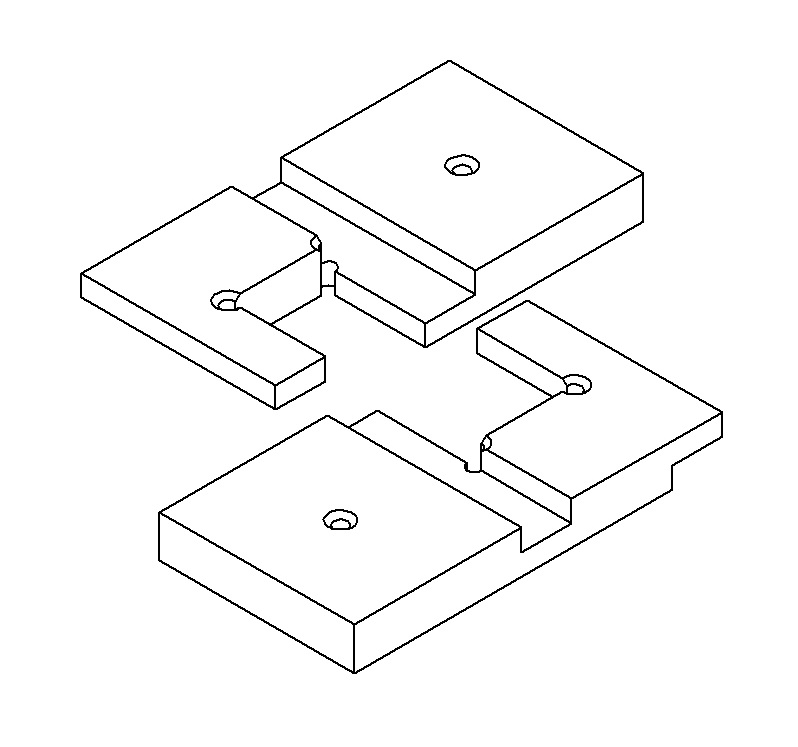
\includegraphics[width=\textwidth]{Hook_iso}
  \caption{Isometric exploded assembly view of proof-of-concept of `The Hook'}
  \label{fig:hook_iso}
\end{figure}

\begin{figure}[h!]
  \centering
  	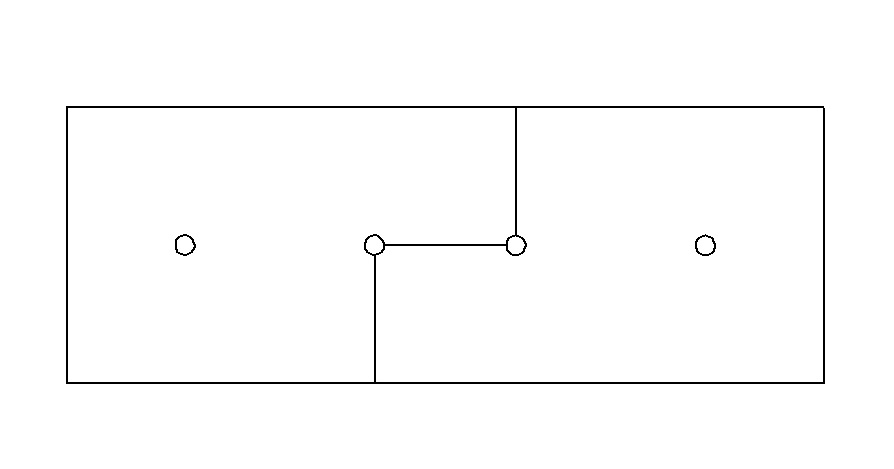
\includegraphics[width=\textwidth]{Hook_top}
  \caption{Top assembly view of proof-of-concept of `The Hook'}
  \label{fig:hook_top}
\end{figure}

\begin{figure}[h!]
  \centering
  	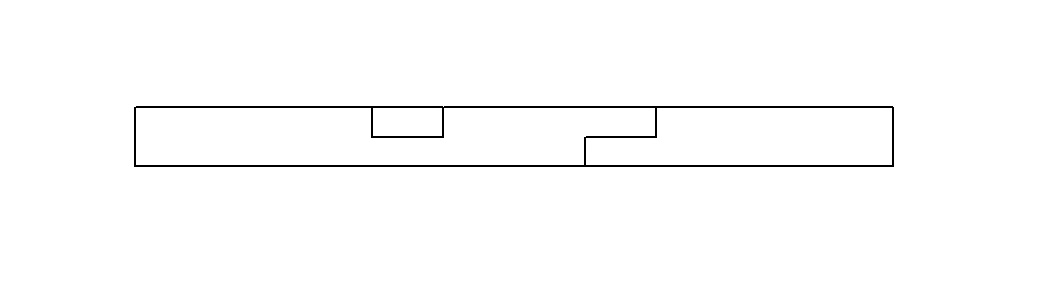
\includegraphics[width=\textwidth]{Hook_right}
  \caption{Right assembly view of proof-of-concept of `The Hook'}
  \label{fig:hook_right}
\end{figure}

The focus of the `The Hook' design is the creation of a fine crack by pushing two plates together. Normally, even though this method yields great results in crack width, the cracks themselves are technically infinitely long (see Section 5.1.4). The Hook design attempts to rectify this issue by using two plates with geometry that allows them to be slotted together. Fig.\ref{fig:hook_iso} roughly shows the concept of such slotting. Once connected, the two pieces form one single layer (the fuselage skin). Fig.\ref{fig:hook_top} shows a portion of such a layer, demonstrating how the crack created would be between two rivets. Additional rivets may be added to each hook piece to provide balance points - while only two more are shown a final design would incorporate more. This assembled layer would be riveted to another sheet (say, a doubler) (not pictured), replicating the repair configuration and keeping the slotted pieces together.

Fig.\ref{fig:hook_right} shows how the thickness of a layer is constant along the length of the crack, and beyond the edge of each slot. In between, though, there is a discontinuity where the two pieces connect vertically. This is a considerable downside as it may affect the signal in unwanted ways.

There would be two hooks per skin layer thickness. Doublers of different thicknesses may interchangeably be fastened to these hooked skin layers. Though only one row of rivets has been shown in the figures, those figures are only an illustration of the slot mechanism; multiple rows of rivets may be incorporated with only minimal change to the geometry.

\clearpage
\subsection{\textsc{The Petri Dish} }

\begin{figure}[h!]
  \centering
  	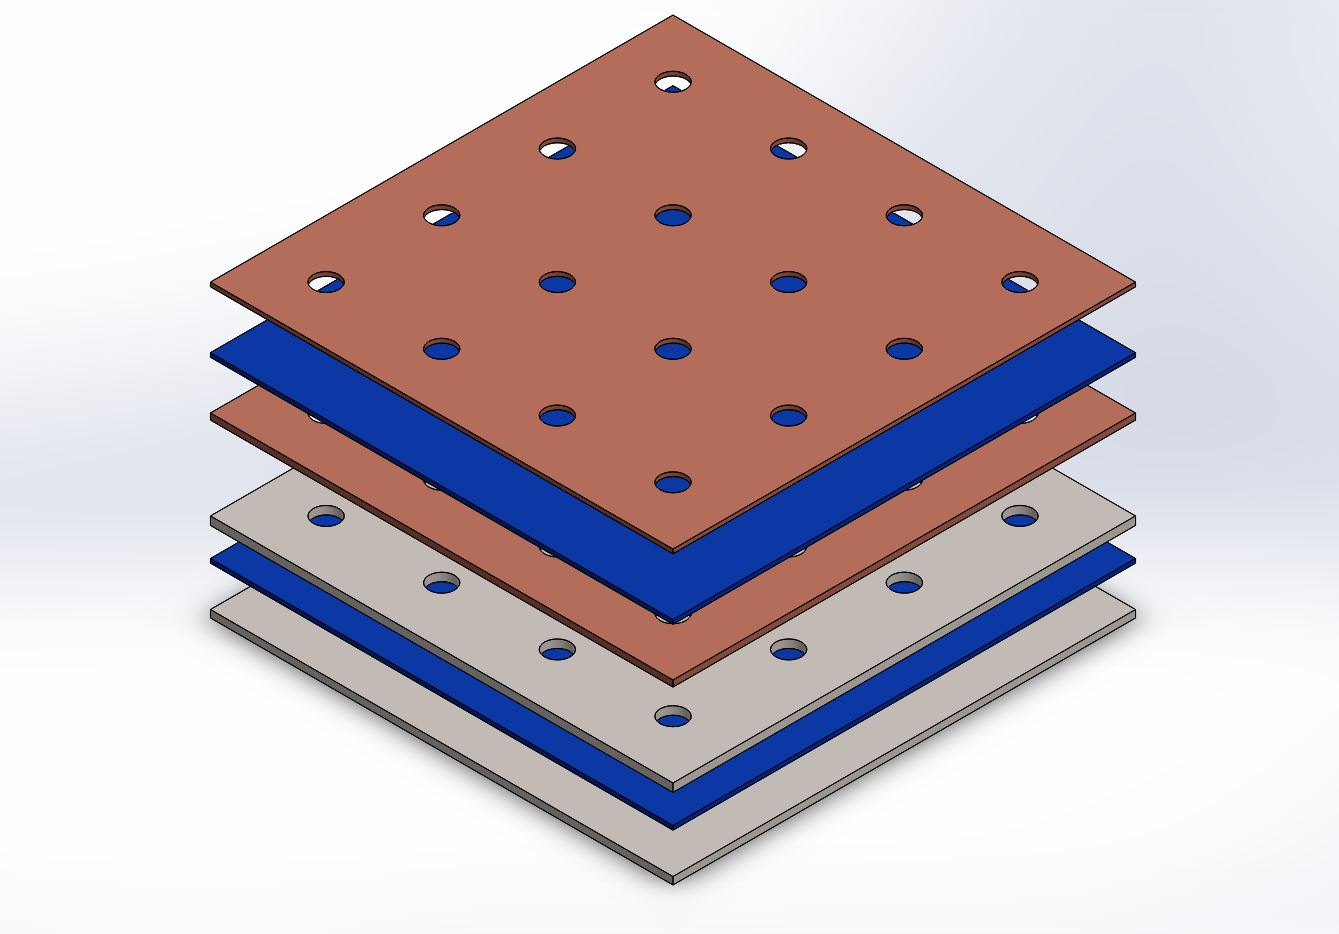
\includegraphics[width=\textwidth]{Petri_iso}
  \caption{Right assembly view of proof-of-concept of `The Petri Dish'}
  \label{fig:petri_iso}
\end{figure}

\begin{figure}[h!]
  \centering
  	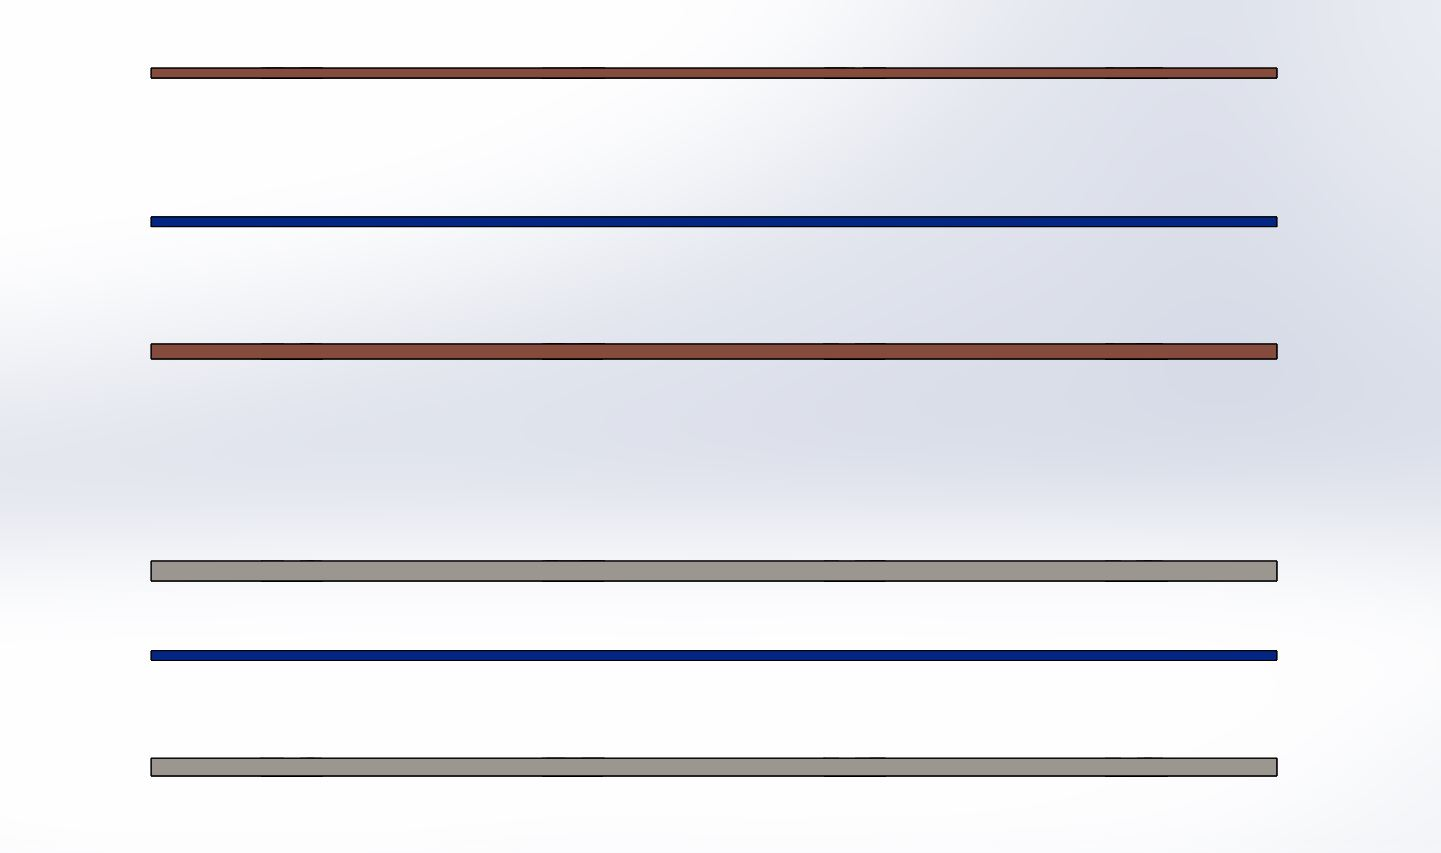
\includegraphics[width=\textwidth]{Petri_left}
  \caption{Right assembly view of proof-of-concept of `The Petri Dish'}
  \label{fig:petri_left}
\end{figure}

The petri dish design basically relies on placing many pieces of metal in close contact with each other to create a larger part. That is to say that if we needed a thick skin then this could be achieved by placing two or more thinner pieces of aluminum on top of each other. The benefit of this design is that we only need a single thin layer of aluminum that contains the crack. This layer can then be moved up or down to shift the crack into either the doubler or the skin or to a specific depth in the skin as required. The issue that was emergent with this design is that we need a non-lossy material that can be applied to the two layers brought into contact - this way the eddy-current does not see significant loss due to the air interface between aluminum layers. There are multiple ways to get around this with suggestions like metal embedded agarose gel, conductive tapes, or a simple salt-solution. In essence the interface-gel should have a conductivity on the same order as that of aluminum (the design can tolerate perhaps an order drop in conductivity). A design should be constrained so that the drop in power should be less than 3dB per assembled part [this can be calculated by $20 \log{\frac{<\rho>}{\rho_{Al}}}$, where $<\rho>$ is the conductivity of entire skin or doubler (the gel layers and the aluminum layers put together)] - the reason for a maximum drop of 3dB is that if we have both the doubler and the skin assemblies at 3dB then in total we would have a drop of 6dB or 50\% attenuation. 

In figures Fig.\ref{fig:petri_iso} and Fig.\ref{fig:petri_left} the gel is represented by the blue layer. The doubler sheets are the brown figures on the top, sandwiching the gel to create a thicker layer. The skin sheets are the grey sheets below, similarly sandwiching a layer of gel. There is no gel between the bottom doubler layer and the top skin layer as air is needed to accurately reflect the double-skin interface. Not pictured are the fasteners that would be in the assembly, and the machined cracks.
\clearpage
\subsection{\textsc{The Staircase} }

\begin{figure}[h!]
  \centering
  	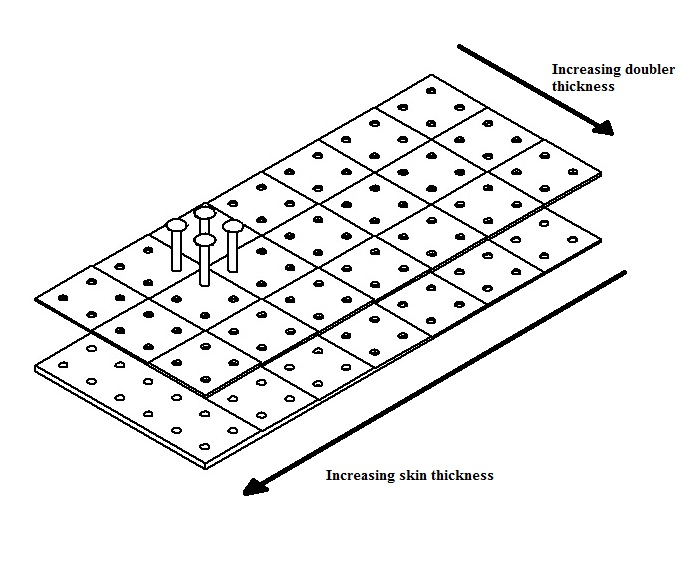
\includegraphics[width=\textwidth]{Steps_iso}
  \caption{Isometric exploded assembly view of `The Staircase'}
  \label{fig:steps_iso}
\end{figure}

\begin{figure}[h!]
  \centering
  	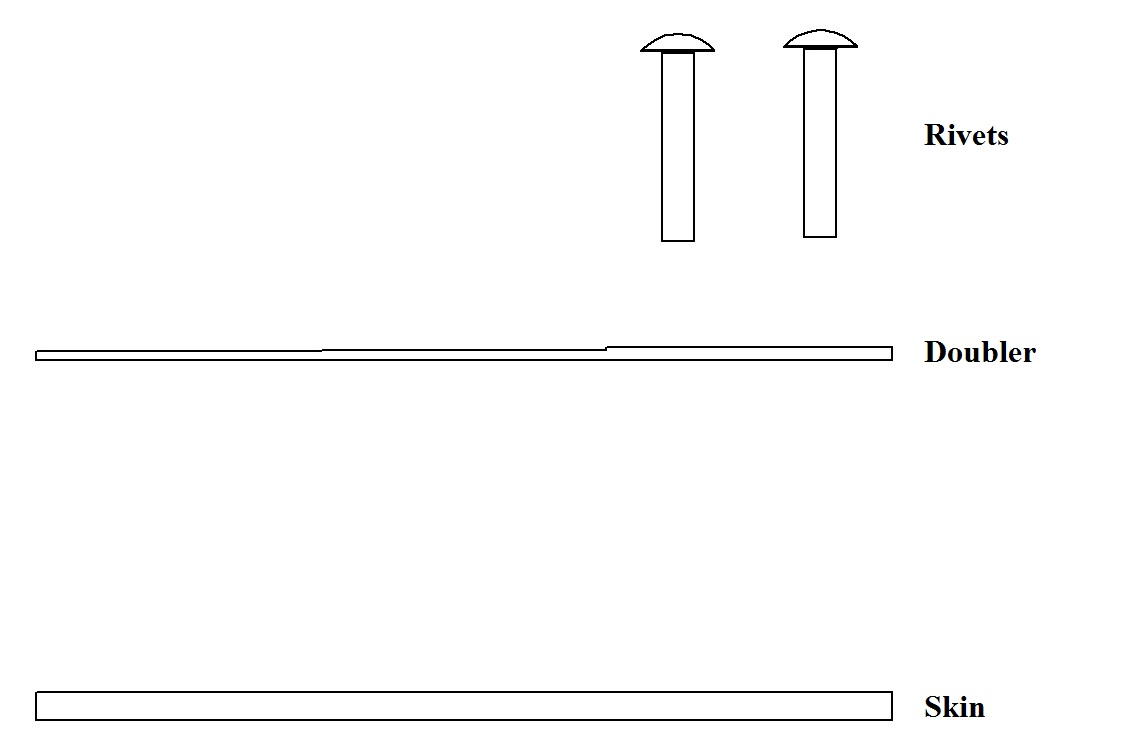
\includegraphics[width=\textwidth]{Steps_front}
  \caption{Front exploded assembly view of `The Staircase'}
  \label{fig:steps_front}
\end{figure}

\begin{figure}[h!]
  \centering
  	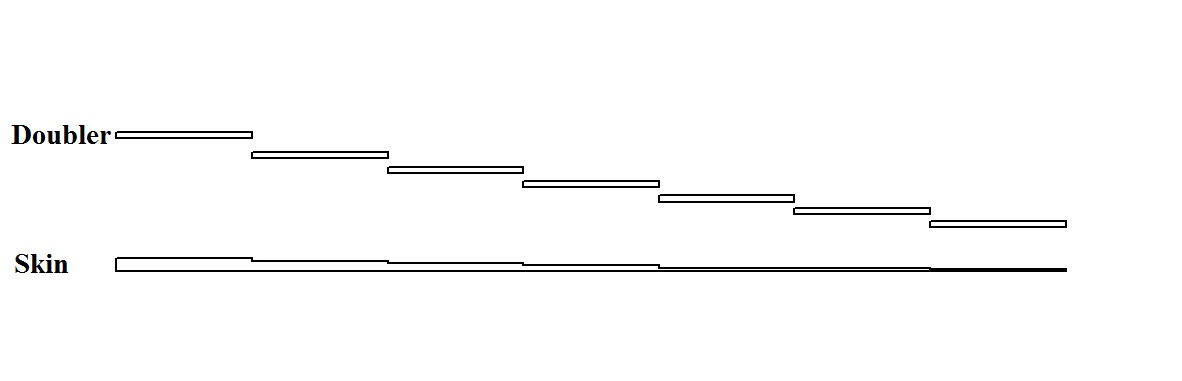
\includegraphics[width=\textwidth]{Steps_right}
  \caption{Right exploded assembly view of `The Staircase'}
  \label{fig:steps_right}
\end{figure}

The staircase design is composed of three major portions;  fuselage skin as a whole with varying thickness,  repair-doubler plates with various thicknesses, and rivets to fasten each repair-doubler plate onto the fuselage skin. The directions of thickness variance is shown in Fig. \ref{fig:steps_iso}.

The fuselage skin is machined from a single block of aluminum. The thickness varies in 7 discrete steps. 12 rivet holes are drilled into each such step as shown in the figure. Cracks can be simulated between two rivets (or a rivet pitch). Each thickness combination has one edge crack propagating from the edge of the body. The skin layer thicknesses can be CNC milled or chemical milled. Other machining methods available are considered too expensive.

As shown in Fig.\ref{fig:steps_right}, the doublers are emulated by 7 separate identical plates with 3 different thicknesses. Each is fastened onto every stair step of the fuselage skin. Hence, one individual plate simulates three doubler thicknesses along one skin thickness.

In conclusion, the aspect of generating various thicknesses is solved in this design by fastening two staircases perpendicular to each other, which creates a total of 21 (3x7) configurations. Cracks can be created on the fuselage skin through laser cutting or EDM.
\newpage

\section{Evaluation \& Final Design}
Now that the alternatives for approaching different design aspects have been chosen, this section will determine the best of the alternatives by way of multi-criterion decision analysis. In this proposal we will be evaluating the designs using a weighted sum model where a number of alternatives are evaluated against each other. It is important to normalize the design features under consideration so that all the parameters have the same unit - for this purpose we are normalizing our design against Bombardier's calibration block, used by operator that we were shown. 

\subsection{\textsc{Finalized Design Criteria}}

Constraints for the project were identified in the project requirements report previously submitted. These constraints and objectives are listed here for the benefit of the reader.

\textbf{Constraints:}
\begin{itemize}
\item Cost
\item Versatility
\item Regulatory compliance
\end{itemize}

Similarly the objectives of the proposed designs are also listed below for the reader. They are listed in order of priority (high to low) along with their normalized weights.

\textbf{Objectives:}
\begin{table}[h!]   
\begin{center}
    \begin{tabular}{ | l | c |}
    \hline
    Selection Criteria & Normalized Weight  \\ \hline
    Low Cost & 0.192    \\ \hline
    Reliability & 0.183    \\ \hline
    Manufacturability & 0.112    \\ \hline
    Ease of Use & 0.112    \\ \hline
    Portability & 0.112    \\ \hline
    Robustness & 0.103    \\ \hline
    Safety & 0.093    \\ \hline
    Traceability & 0.093    \\ \hline
	\end{tabular}
\caption{Table showing the normalized weight ascribed by the team to a given objective}
\label{norm}    
\end{center}
\end{table}

Due to the low priority the team gave to ergonomics (a score of 1.5 out of a maximum of 5) in the project requirements, it has been decided that the objective be dropped for the purposes of evaluation. As such ergonomics will not be a deciding factor between alternatives.


\subsection{\textsc{Weighted Sum Model}}
In general, with normalized features, the value of a specific design '$A$' can be given by: $$A^{WSM-score} = \sum_{j=1}^n {w_j \sum^{m_n}_{k=1} {u_{jk} a_{jk}}}$$ where $w_j$ is the normalized weight given to a particular objective '$j$' and $u_{jk}$ is the relative importance of a particular design feature '$k$' to the given objective, and $a_{jk}$ is the value of the design feature '$k$' evaluated against objective '$j$'. The total number of objectives is $n$ and the total number of features relating to that objective is $m_n$. The weights $w_j$ were decided in the project proposal and the normalized values are shown in Table. \ref{norm}. The weights $u_{jk}$ are shown in Table. \ref{table1} in the Appendix along with the features and their relative values $a_{jk}$.

\begin{table}[h!]   
\begin{center}
    \begin{tabular}{ | l | c |}
    \hline
    Proposed Design & Weighted Sum Minimization Score  \\ \hline
    The Staircase & 0.8597    \\ \hline
    The Petri Dish & 0.8642    \\ \hline
    The Hook & 0.9051    \\ \hline
	\end{tabular}
\caption{Table showing Proposed Designs and their Weighted Sum Minimization Scores}
\label{results}    
\end{center}
\end{table}

\subsection{\textsc{Modifications to the final design}}

After optimization and decision analysis, Section 7.2 shows that the optimal design to be implemented is the `Staircase' design. The additional cost of the multiple cracks is countered by the higher reliability and ease of use. After conferring with the client, significant changes to the `Staircase' design were made and are illustrated in Fig. \ref{fig:staircase_mod}.

\begin{figure}[h!]
  \centering
  	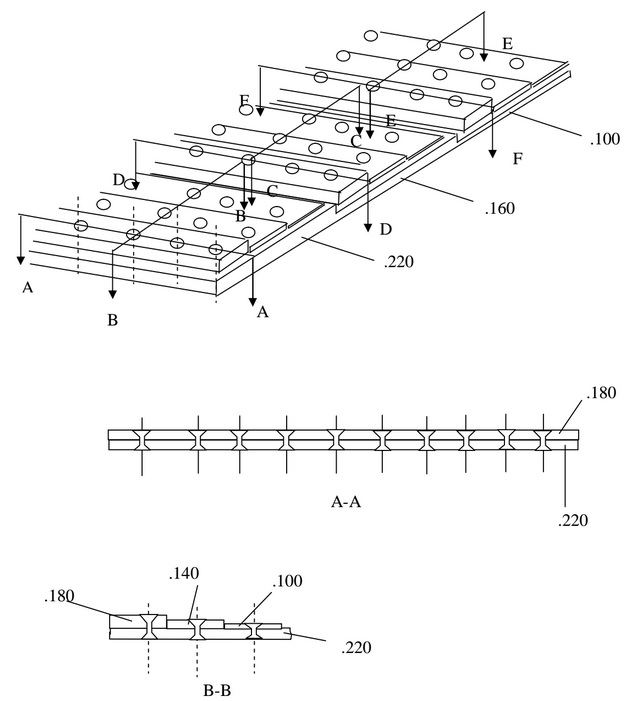
\includegraphics[width=\textwidth]{staircase_mod}
  \caption{Modified `Staircase' design}
  \label{fig:staircase_mod}
\end{figure}

The staircase portion of the design (representing the air-craft skin) now has only three steps, or, thicknesses. Onto each step three different thicknesses of repair-doubler are fastened. Cracks are simulated by EDM between sets of two rivets on both the fuselage skin and repair doubler plates. Per each step of the staircase three types of cracks are generated: three surface cracks, three subsurface cracks, and two cracks on the surface of the fuselage skin spanning different doubler thicknesses. This simulates eight configurations per step of fuselage skin, totalling twenty-four configurations per calibration block. The whole calibration block has ninety rivet locations, thirty per fuselage skin thickness. 

\clearpage
\section{Cost Analysis of Final Design}

The cost per part can be estimated from the costs incurred by the team in making a proof-of-
concept prototype. For example, the cost of aluminum was found through the same provider of the 12''x12''x0.16'' aluminum sheet used to make a third of the universal block. The price shown below is for a 12''x12''x0.25'' aluminum sheet, with which the whole calibration block may be made.

It should be noted that due to economies of scale in the mass production process, the costs involved should be significantly reduced. Cost differences generated by  variations in the materials used for the skin or doubler should be relatively minimal. The  total cost of the final design is shown in the table below. Machining costs have been taken from quotes available in the Appendix. 

\vspace{10mm}

\begin{table}[H]
\centering
\begin{tabular}{@{}ll@{}}
\toprule
\rowcolor[HTML]{C0C0C0} 
\textbf{Raw material breakdown}   &                     \\ \midrule
Aluminium 2024-T3 clad 12''x12''x0.25''    & \$ 82.92            \\
Rivets                            & \$ 9.01             \\ \midrule
\rowcolor[HTML]{C0C0C0} 
\textbf{Machining cost breakdown} & \textbf{}           \\ \midrule
Waterjet cutting and CNC milling  & \$ 206.25           \\
EDM Notches ($85 or $65/notch)    & \$ 2310.00          \\ \midrule
\rowcolor[HTML]{C0C0C0} 
\textbf{Total Cost}               & \textbf{\$ 2608.18} \\ \bottomrule
\end{tabular}
\caption{Table showing cost breakdown of Final Design}
\end{table}

\newpage
\section{Removable Fasteners}

During the design review and critique, Bombardier Aerospace had the team consider making the rivets in the design be removable. This would allow operators to use different types of rivets on the same calibration block. In response to this, the team has proposed purchasing countersunk rivets longer than the doubler/skin thicknesses, and then threading them. The external threads may be made by simply using a manual die. Then, the rivets may be held in place by a nut, instead of having to be permanently riveted in.

Furthermore, the use of removable rivets makes it possible to replace parts of the design should they be damaged. This would not be possible otherwise, not without further damaging the components.

This solution utilizes simple manufacturing/machining methods and common components, making it simple to implement. The use of this design can be explored further in the future to see the extent to which it affects the probe signal and calibration (if at all).
\newpage

\section{Appendix}
%\addcontentsline{toc}{section}{Appendix}
\subsection{\textsc{Notes from phone call with Mr. Vinitsky}}
The following are notes taken from a call made to Alex Vinitsky on October 30th, 2014, to clarify and expand upon the topics covered in a group meeting on October 7th, 2014.

\begin{itemize}
\item only major companies have NDT departments/devoted NDT specialists
\item most companies rent/contract out this inspection work
\item Level 2 and Level 1 NDT specialists are the actual end-users, they're the ones who carry out the inspections
\item Airlines usually outsource maintenance activity
\begin{itemize}
\item For example, apparently Air Canada ten years back made their maintenance section a different company altogether, and then just went and outsourced their maintenance work with cheaper companies. Note: Details may not be correct. 
\end{itemize}
\item So, in general, airlines outsource their maintenance a lot
\item They're concerned with making sure accreditation is current
\item Our blocks are for repairs, though. These repairs usually have a threshold of 40,000 flight cycles, after which repair parts are deemed to be at the ends of their lives. By that time, though, plane is usually with a different operator
\begin{itemize}
\item New operators tend to deal with approaching thresholds last minute
\item Bombardier (and companies like it) ship in relevant calibration blocks
\end{itemize}
\item When not in use, the calibration blocks are just lying on shelves in some room NDT engineers keep for themselves.
\begin{itemize}
\item They usually move the blocks around in foam cases
\item Still, no sharp corners on the blocks is requested
\end{itemize}
\item Because they're shipped, these blocks get lost a lot! Sometimes they're sent back to the wrong department in Bombardier
\begin{itemize}
\item  Giving the final design a part number or serial number on it helps, traceability would be a nice feature
\end{itemize}
\end{itemize}

\subsection{\textsc{Design Features and Objectives}}
% Please add the following required packages to your document preamble:
% \usepackage{graphicx}
% \usepackage[table,xcdraw]{xcolor}
% If you use beamer only pass "xcolor=table" option, i.e. \documentclass[xcolor=table]{beamer}
\begin{table}[h]
\centering
\caption{Table showing design features and scores as related to objectives}
\label{table1}
\resizebox{\textwidth}{!}{%
\begin{tabular}{rllll}
\multicolumn{1}{l}{\textbf{}}                  & \textbf{The Staircase}                                            & \textbf{The Petri Dish}                                           & \textbf{The Hook}                                                 & \textbf{Bombardier's CTS} \\ \cline{2-5} 
\multicolumn{1}{l}{\textbf{Cost}}              &                                                                   &                                                                   &                                                                   &                           \\ \cline{1-1}
Number of cracks                               & 42                                                                & 2                                                                 & 0                                                                 & 17                        \\
Number of processes (ignoring EDM)             & 3                                                                 & 3                                                                 & 4                                                                 & 3                         \\
\rowcolor[HTML]{C0C0C0} 
\textit{Normalized Cost of Crack}              & \multicolumn{1}{r}{\cellcolor[HTML]{C0C0C0}\textit{2.470588235}}  & \multicolumn{1}{r}{\cellcolor[HTML]{C0C0C0}\textit{0.1176470588}} & \multicolumn{1}{r}{\cellcolor[HTML]{C0C0C0}\textit{0}}            & \textit{}                 \\
\rowcolor[HTML]{C0C0C0} 
\textit{Number of Processes}                   & \multicolumn{1}{r}{\cellcolor[HTML]{C0C0C0}\textit{1}}            & \multicolumn{1}{r}{\cellcolor[HTML]{C0C0C0}\textit{1}} & \multicolumn{1}{r}{\cellcolor[HTML]{C0C0C0}\textit{1.333333333}}  & \textit{}                 \\
\multicolumn{1}{l}{}                           &                                                                   &                                                                   &                                                                   &                           \\
\multicolumn{1}{l}{\textbf{Safety}}            &                                                                   &                                                                   &                                                                   &                           \\ \cline{1-1}
Team Member 1                                  & 8                                                                 & 7                                                                 & 10                                                                & 8                         \\
Team Member 2                                  & 10                                                                & 7                                                                 & 7                                                                 & 10                        \\
Team Member 3                                  & 8                                                                 & 7                                                                 & 7                                                                 & 10                        \\
Team Member 4                                  & 9                                                                 & 6                                                                 & 9                                                                 & 10                        \\
Avg. Value                                     & 8.75                                                              & 6.75                                                              & 8.25                                                              & 9.333333333               \\
\rowcolor[HTML]{C0C0C0} 
\textit{Normalized and Reciprocal Safety Value}               & \multicolumn{1}{r}{\cellcolor[HTML]{C0C0C0}\textit{1.0667}}       & \multicolumn{1}{r}{\cellcolor[HTML]{C0C0C0}\textit{1.3827}} & \multicolumn{1}{r}{\cellcolor[HTML]{C0C0C0}\textit{1.1313}} & \textit{}                 \\
\multicolumn{1}{l}{}                           &                                                                   &                                                                   &                                                                   &                           \\
\multicolumn{1}{l}{\textbf{Portability}}       &                                                                   &                                                                   &                                                                   &                           \\ \cline{1-1}
Volume                                         & 20.46                                                             & 9.75                                                              & 3.41                                                              & 20                        \\
Surface Area                                   & 446                                                               & 95                                                                & 111.5                                                             & 400                       \\
Volume/Surface Area                            & 0.04587443946                                                     & 0.1026315789                                                      & 0.03058295964                                                     & 0.05                      \\
\rowcolor[HTML]{C0C0C0} 
\textit{Normalized Reciprocal Portability measure}         & \multicolumn{1}{r}{\cellcolor[HTML]{C0C0C0}\textit{1.090}} & \multicolumn{1}{r}{\cellcolor[HTML]{C0C0C0}\textit{0.4872}}  & \multicolumn{1}{r}{\cellcolor[HTML]{C0C0C0}\textit{1.6349}} & \textit{}                 \\
\multicolumn{1}{l}{}                           &                                                                   &                                                                   &                                                                   &                           \\
\multicolumn{1}{l}{\textbf{Ease of Use}}       &                                                                   &                                                                   &                                                                   &                           \\ \cline{1-1}
Number of individual parts                     & 8                                                                 & 13                                                                & 17                                                                & 8                         \\
Approximate Set-up time                        & 0                                                                 & 14                                                                 & 13.75                                                             &                           \\
\rowcolor[HTML]{C0C0C0} 
\textit{Normalized Part}                       & \multicolumn{1}{r}{\cellcolor[HTML]{C0C0C0}\textit{1}}            & \multicolumn{1}{r}{\cellcolor[HTML]{C0C0C0}\textit{1.625}}        & \multicolumn{1}{r}{\cellcolor[HTML]{C0C0C0}\textit{2.125}}        & \textit{}                 \\
\rowcolor[HTML]{C0C0C0} 
\textit{Normalized Set-Up Time}                & \multicolumn{1}{r}{\cellcolor[HTML]{C0C0C0}\textit{0}}            & \multicolumn{1}{r}{\cellcolor[HTML]{C0C0C0}\textit{1.4}}          & \multicolumn{1}{r}{\cellcolor[HTML]{C0C0C0}\textit{1.375}}        & \textit{}                 \\
\multicolumn{1}{l}{}                           &                                                                   &                                                                   &                                                                   &                           \\
\multicolumn{1}{l}{\textbf{Reliability}}       &                                                                   &                                                                   &                                                                   &                           \\ \cline{1-1}
\rowcolor[HTML]{C0C0C0} 
\textit{Reliability of Thickness Generation}   & \multicolumn{1}{r}{\cellcolor[HTML]{C0C0C0}\textit{0}}            & \multicolumn{1}{r}{\cellcolor[HTML]{C0C0C0}\textit{0.64}}        & \multicolumn{1}{r}{\cellcolor[HTML]{C0C0C0}\textit{1.33}}        & \textit{}                \\

\rowcolor[HTML]{C0C0C0} 
\textit{Probability of Error Propagation}   & \multicolumn{1}{r}{\cellcolor[HTML]{C0C0C0}\textit{0}}            & \multicolumn{1}{r}{\cellcolor[HTML]{C0C0C0}\textit{1}}        & \multicolumn{1}{r}{\cellcolor[HTML]{C0C0C0}\textit{0.4}}        & \textit{}                \\

\multicolumn{1}{l}{}                           &                                                                   &                                                                   &                                                                   &                           \\
\multicolumn{1}{l}{\textbf{Traceability}}      &                                                                   &                                                                   &                                                                   &                           \\ \cline{1-1}
\rowcolor[HTML]{C0C0C0} 
\textit{Binary Inverted Traceability Measure}           & \multicolumn{1}{r}{\cellcolor[HTML]{C0C0C0}\textit{0}}            & \multicolumn{1}{r}{\cellcolor[HTML]{C0C0C0}\textit{1}}            & \multicolumn{1}{r}{\cellcolor[HTML]{C0C0C0}\textit{0}}            &                          \\
\multicolumn{1}{l}{}                           &                                                                   &                                                                   &                                                                   &                           \\
\multicolumn{1}{l}{\textbf{Robustness}}        &                                                                   &                                                                   &                                                                   &                           \\ \cline{1-1}
Surface Area                                   & 446                                                               & 95                                                                & 111.5                                                             & 400                       \\
\rowcolor[HTML]{C0C0C0} 
\textit{Normalized Surface Area}               & \multicolumn{1}{r}{\cellcolor[HTML]{C0C0C0}\textit{1.115}}        & \multicolumn{1}{r}{\cellcolor[HTML]{C0C0C0}\textit{0.2375}}       & \multicolumn{1}{r}{\cellcolor[HTML]{C0C0C0}\textit{0.27875}}      & \textit{}                 \\
\multicolumn{1}{l}{}                           &                                                                   &                                                                   &                                                                   &                           \\
\multicolumn{1}{l}{\textbf{Manufacturability}} &                                                                   &                                                                   &                                                                   &                           \\ \cline{1-1}
Number of Manufacturing Processes used.    & 4                                                                 & 4                                                                 & 5                                                                 & 4                         \\
\rowcolor[HTML]{C0C0C0} 
\textit{Normalized Number of Processes}        & \multicolumn{1}{r}{\cellcolor[HTML]{C0C0C0}\textit{1}}            & \multicolumn{1}{r}{\cellcolor[HTML]{C0C0C0}\textit{1}}         & \multicolumn{1}{r}{\cellcolor[HTML]{C0C0C0}\textit{1.25}}         & \textit{}                
\end{tabular}
}
\end{table}

\newpage
\subsection{\textsc{Digital Precision EDM Quote}}


\begin{figure}[h!]
  \centering
  	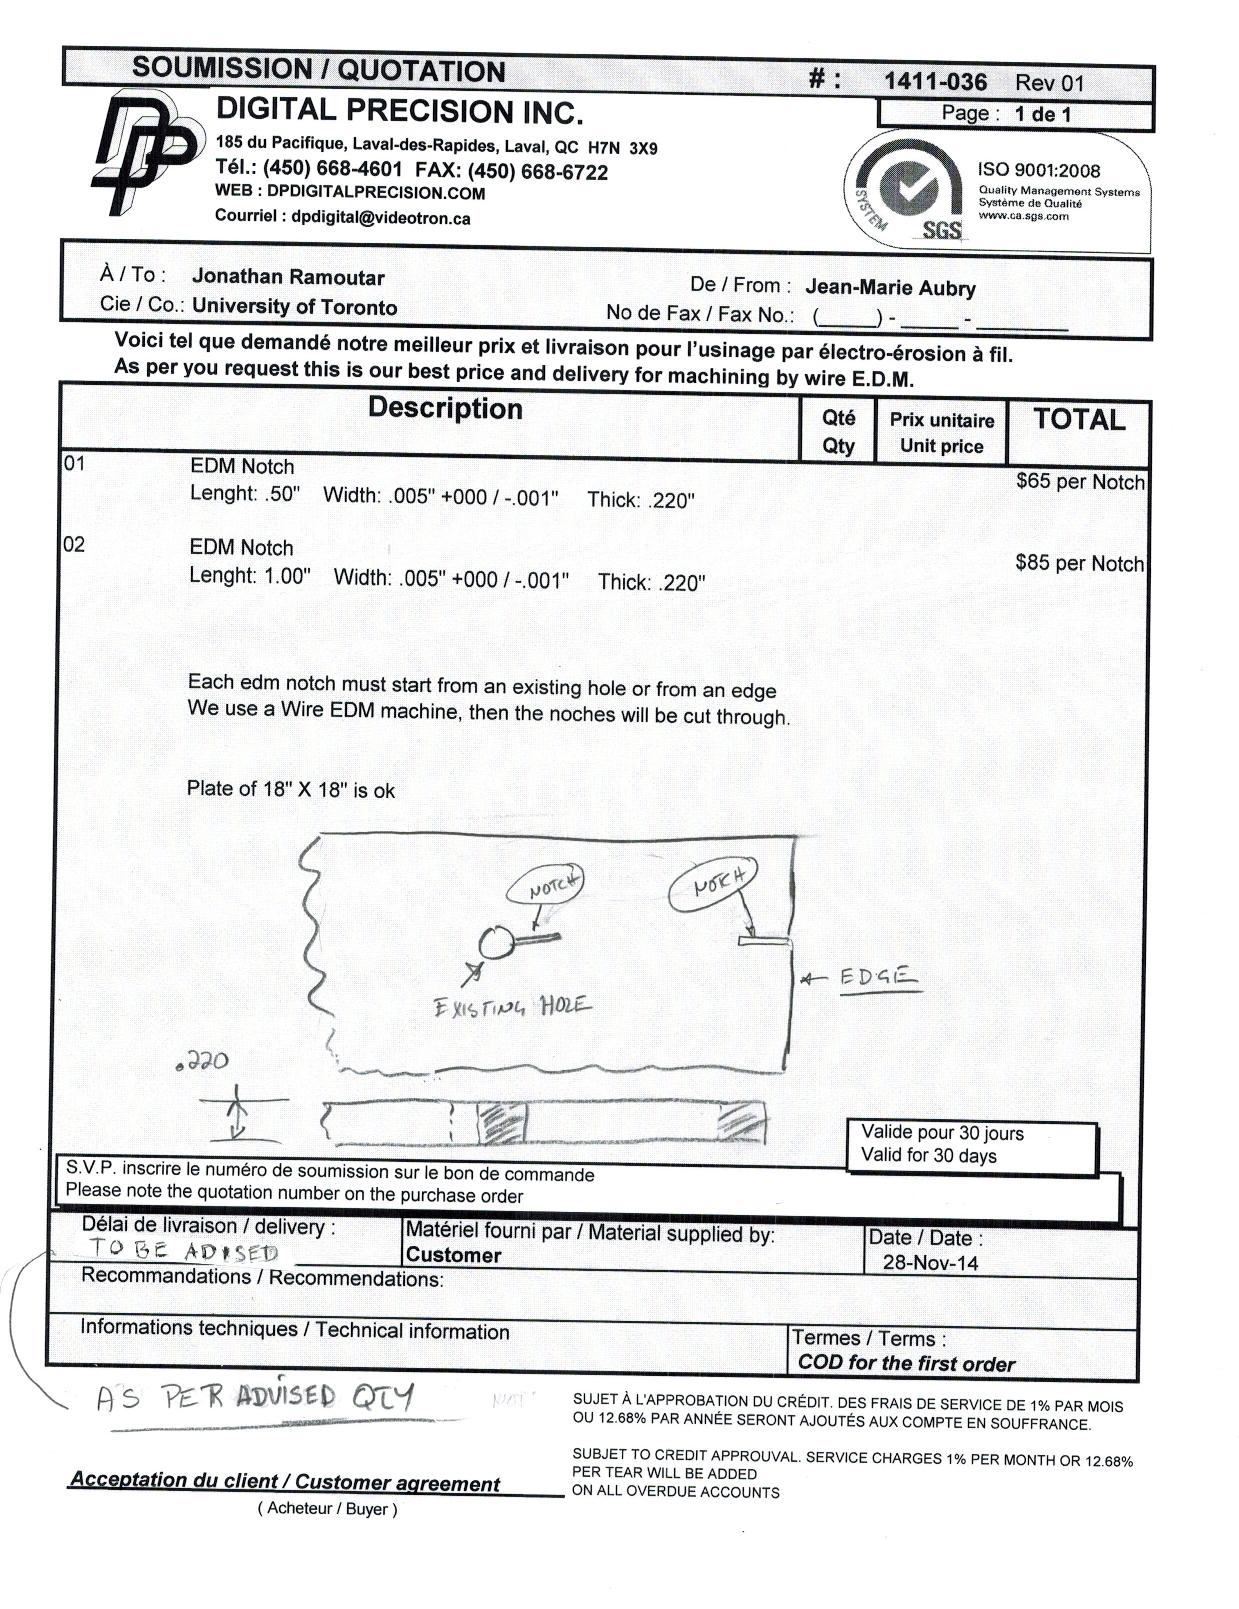
\includegraphics[width=0.95\textwidth]{quote.pdf}
  \label{fig:quote}
\end{figure}

\subsection{\textsc{Machining Quote}}

\begin{figure}[h!]
  \centering
  	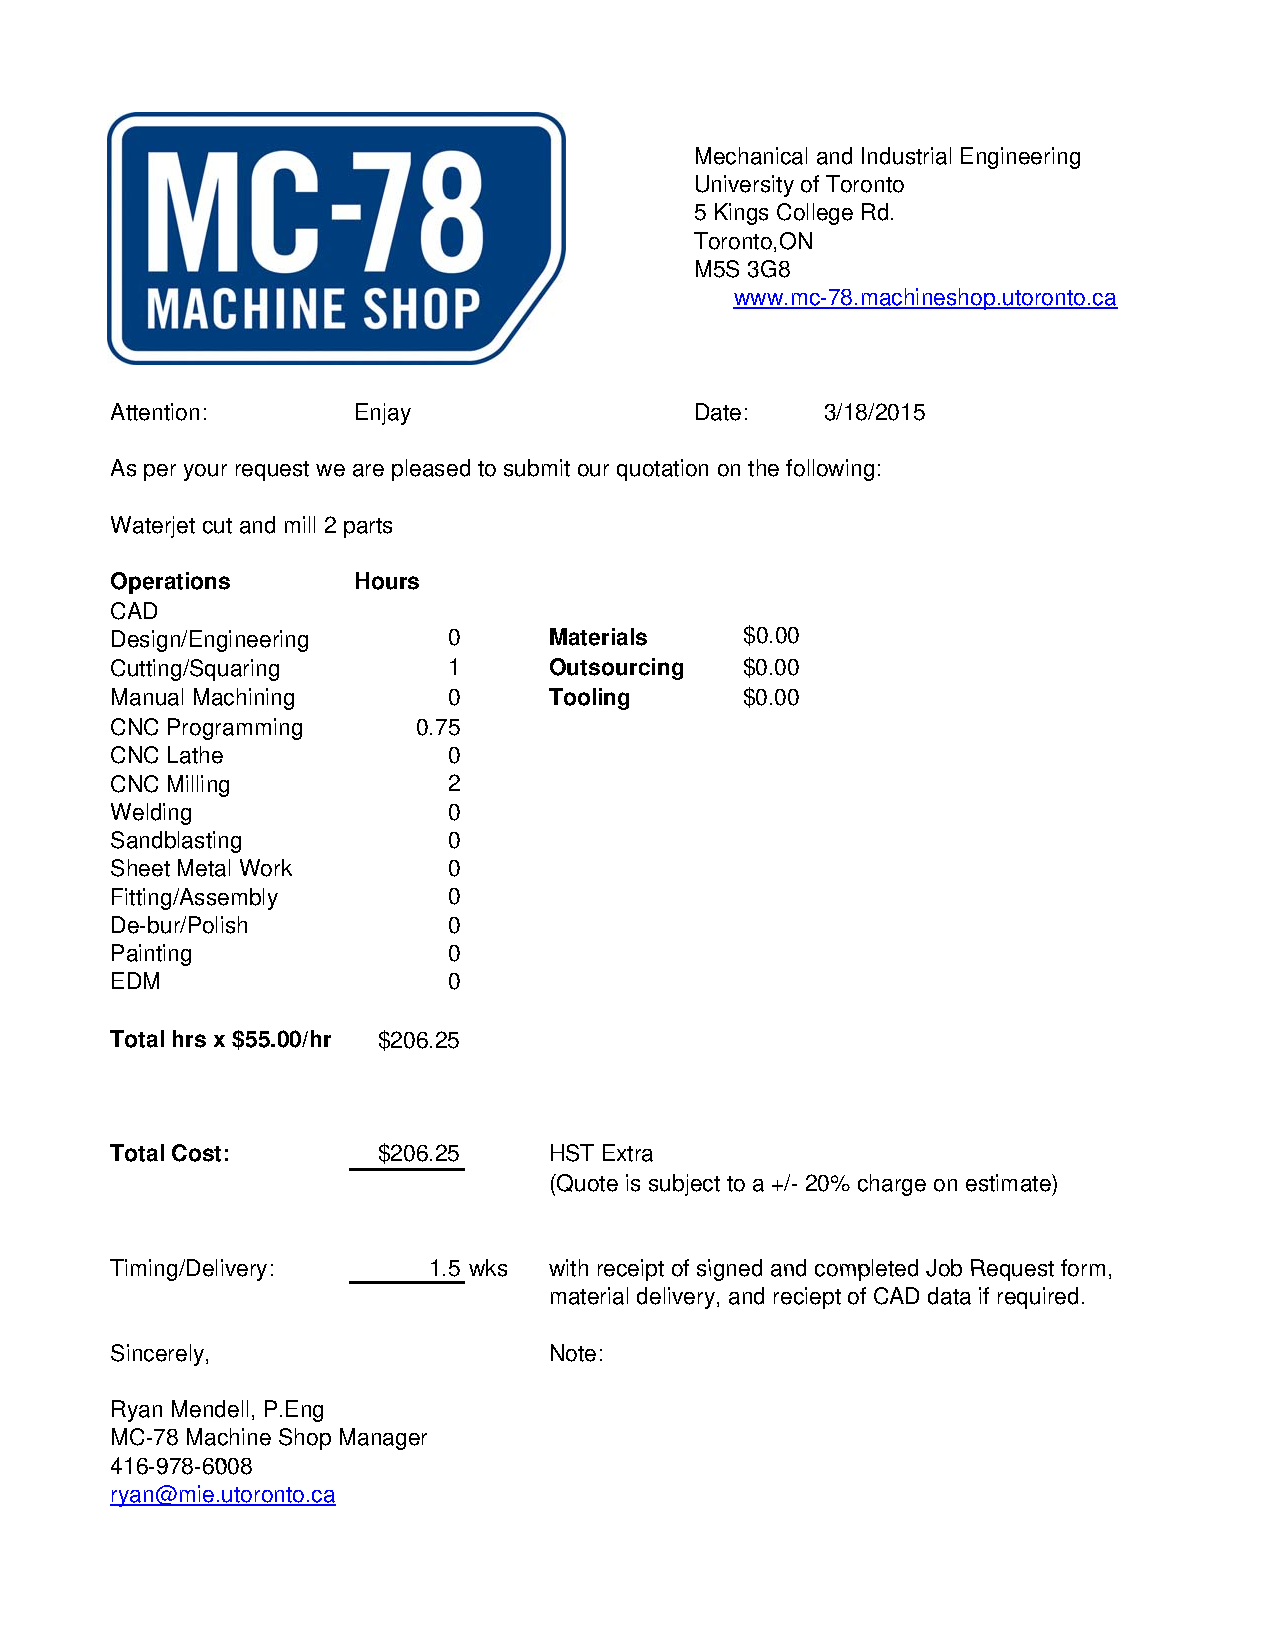
\includegraphics[width=0.95\textwidth]{MCQuote.pdf}
  \label{fig:mcquote}
\end{figure}

%-------------------------------------------------------------------------------
% REFERENCES
%-------------------------------------------------------------------------------
\newpage

\section*{References}
\addcontentsline{toc}{section}{References}

\noindent
[1] INTERNATIONAL ATOMIC ENERGY AGENCY, Eddy Current Testing at Level 2: Manual for the Syllabi Contained IAEA-TECDOC-628/Rev. 2 `Training Guidelines for Non-Destructive Testing Techniques', 1st ed. Vienna: IAEA, 2011, pp. 7-9.
\newline
\newline
\noindent
[2] J. Schijve, `Four lectures on fatigue crack growth', Engineering Fracture Mechanics, vol. 11, no. 1, pp. 167--168, 1979.
\newline
\newline
\noindent
[3] G. Sih, `Multiscale approach to micro/macro fatigue crack growth in 2024-T3 aluminum panel', Science China Physics, Mechanics and Astronomy, vol. 57, no. 1, pp. 51--58, 2014.
\newline
\newline
\noindent
[4] J. Newman Jr, `Advances in fatigue and fracture mechanics analyses for metallic aircraft structures', NASA Langley technical report server, 2000.
\newline
\newline
\noindent
[5] J. Schijve, F. Jacobs and P. Tromp, Crack Propagation in Aluminum Alloy Sheet Materials under Flight-Simulation Loading. Ft. Belvoir: Defense Technical Information Center, 1970.
\newline
\newline
\noindent
[6] MicroChemicals, 'Aluminium Etching', 2014. [Online]. Available: http://microchemicals. com/technical \_information/aluminium\_etching.pdf. [Accessed: 29- Nov- 2014].
\newline
\newline
\noindent
[7] K. Williams, K. Gupta and M. Wasilik, 'Etch rates for micromachining processing-part II', J. Microelectromech. Syst., vol. 12, no. 6, pp. 761-778, 2003.
\newline
\newline
\noindent
[8] Custompartnet.com, 'Machining Cost Estimator', 2014. [Online]. Available: http://www. custompartnet.com/estimate/machining/. [Accessed: 29- Nov- 2014].
\newline
\newline
\noindent
[9] Jobshop.com, 'Chemical Milling on JobShop.com', 2014. [Online]. Available: http://www. jobshop.com/techinfo/papers/chemmillpaper.shtml. [Accessed: 29- Nov- 2014].
\newline
\newline
\noindent


\end{document}
